\documentclass[tikz,border=8pt]{standalone}
% Shared look for every TikZ diagram. Load with % Shared look for every TikZ diagram. Load with % Shared look for every TikZ diagram. Load with \input{../../tools/tikz-style.tex}
\usepackage[T1]{fontenc}
\usepackage{lmodern}
\renewcommand{\sfdefault}{lmr}  % diagrams use the same serif as the text
\usetikzlibrary{arrows.meta, positioning, shapes.geometric, calc, fit, backgrounds}
\definecolor{cblue}{HTML}{4C78A8}
\definecolor{corange}{HTML}{F58518}
\definecolor{cgreen}{HTML}{54A24B}
\definecolor{cred}{HTML}{E45756}
\definecolor{cpurple}{HTML}{B279A2}
\definecolor{cgrey}{HTML}{6B6B6B}
\tikzset{
  every picture/.style={font=\sffamily, line width=1.2pt},
  box/.style={draw=#1, fill=#1!12, rounded corners=4pt, align=center, inner sep=7pt, minimum height=1.1cm},
  box/.default=cgrey,
  arrow/.style={-{Stealth[length=3mm]}, draw=cgrey, line width=1.4pt},
  title/.style={font=\sffamily\bfseries\Large},
  note/.style={font=\sffamily\small, text=cgrey, align=center},
}
\AtBeginDocument{\hyphenpenalty=10000 \exhyphenpenalty=10000}

\usepackage[T1]{fontenc}
\usepackage{lmodern}
\renewcommand{\sfdefault}{lmr}  % diagrams use the same serif as the text
\usetikzlibrary{arrows.meta, positioning, shapes.geometric, calc, fit, backgrounds}
\definecolor{cblue}{HTML}{4C78A8}
\definecolor{corange}{HTML}{F58518}
\definecolor{cgreen}{HTML}{54A24B}
\definecolor{cred}{HTML}{E45756}
\definecolor{cpurple}{HTML}{B279A2}
\definecolor{cgrey}{HTML}{6B6B6B}
\tikzset{
  every picture/.style={font=\sffamily, line width=1.2pt},
  box/.style={draw=#1, fill=#1!12, rounded corners=4pt, align=center, inner sep=7pt, minimum height=1.1cm},
  box/.default=cgrey,
  arrow/.style={-{Stealth[length=3mm]}, draw=cgrey, line width=1.4pt},
  title/.style={font=\sffamily\bfseries\Large},
  note/.style={font=\sffamily\small, text=cgrey, align=center},
}
\AtBeginDocument{\hyphenpenalty=10000 \exhyphenpenalty=10000}

\usepackage[T1]{fontenc}
\usepackage{lmodern}
\renewcommand{\sfdefault}{lmr}  % diagrams use the same serif as the text
\usetikzlibrary{arrows.meta, positioning, shapes.geometric, calc, fit, backgrounds}
\definecolor{cblue}{HTML}{4C78A8}
\definecolor{corange}{HTML}{F58518}
\definecolor{cgreen}{HTML}{54A24B}
\definecolor{cred}{HTML}{E45756}
\definecolor{cpurple}{HTML}{B279A2}
\definecolor{cgrey}{HTML}{6B6B6B}
\tikzset{
  every picture/.style={font=\sffamily, line width=1.2pt},
  box/.style={draw=#1, fill=#1!12, rounded corners=4pt, align=center, inner sep=7pt, minimum height=1.1cm},
  box/.default=cgrey,
  arrow/.style={-{Stealth[length=3mm]}, draw=cgrey, line width=1.4pt},
  title/.style={font=\sffamily\bfseries\Large},
  note/.style={font=\sffamily\small, text=cgrey, align=center},
}
\AtBeginDocument{\hyphenpenalty=10000 \exhyphenpenalty=10000}

\begin{document}
% Section 3: self-attention without positions. The two sentences contain the same four embeddings, so self-attention
% returns the same four output vectors, only in a different order; "lion" gets the same output in both.
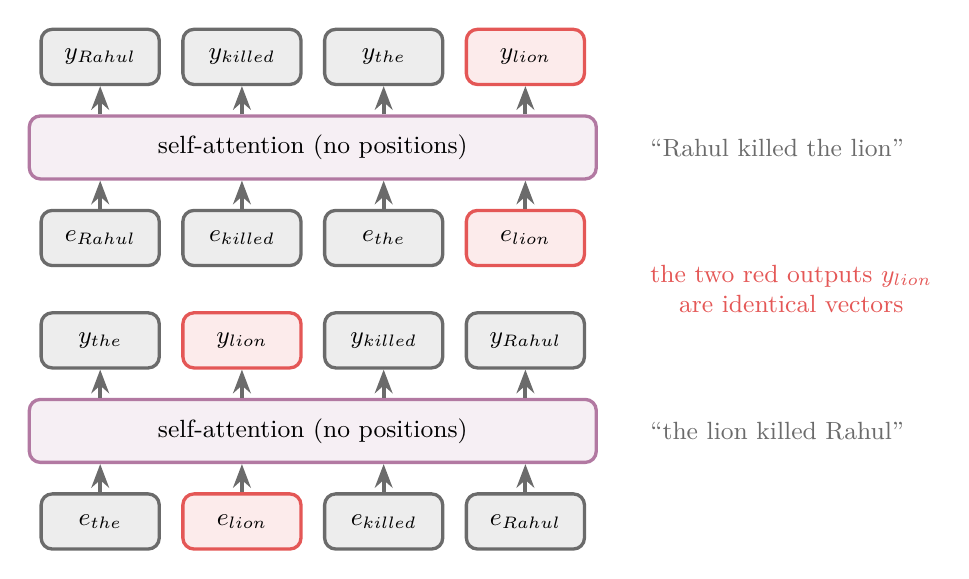
\begin{tikzpicture}[w/.style={box=#1, minimum width=1.5cm, minimum height=0.7cm, inner sep=2pt, font=\sffamily\small},
  sa/.style={draw=cpurple, fill=cpurple!12, rounded corners=4pt, minimum width=7.2cm, minimum height=0.8cm, font=\sffamily\small}]
  \foreach \row/\y/\words in {0/0/{Rahul,killed,the,lion}, 1/-3.6/{the,lion,killed,Rahul}} {
    \node[sa] (sa\row) at (3.75, \y) {self-attention (no positions)};
    \foreach \w [count=\i] in \words {
      \def\c{cgrey}\ifnum\pdfstrcmp{\w}{lion}=0 \def\c{cred}\fi
      \node[w=\c] (x\row\i) at (1.8*\i - 0.75, \y - 1.15) {$e_{\text{\w}}$};
      \node[w=\c] (y\row\i) at (1.8*\i - 0.75, \y + 1.15) {$y_{\text{\w}}$};
      \draw[arrow] (x\row\i) -- (x\row\i |- sa\row.south);
      \draw[arrow] (y\row\i |- sa\row.north) -- (y\row\i);
    }
  }
  \node[note, anchor=west] at (7.9, 0) {``Rahul killed the lion''};
  \node[note, anchor=west] at (7.9, -3.6) {``the lion killed Rahul''};
  \node[note, anchor=west, text=cred] at (7.9, -1.8) {the two red outputs $y_{\text{lion}}$\\are identical vectors};
\end{tikzpicture}
\end{document}
